%% Zweiseitiges Layout
\documentclass[11pt,twoside,a4paper,fleqn]{report}
\usepackage[top=3cm, bottom=2.5cm, left=4cm, right=3cm]{geometry}

%% Schriftbild
\usepackage{lmodern}  % Latin Modern Zeichensatz
\usepackage[utf8]{inputenc}  % Unterstützung von Umlauten im Quelltext
\usepackage[T1]{fontenc}  % Korrekte Umlaute im PDF
\usepackage[english]{babel}  % Silbentrennung nach neuer Rechtschreibung
\renewcommand{\familydefault}{\sfdefault}  % Serifenlose Schrift
\usepackage{setspace}\onehalfspacing  % 1.5-facher Zeilenabstand
\renewcommand{\arraystretch}{1.5}  % 1.5-facher Zeilenabstand (Tabellen)
\setlength{\parindent}{0pt}  % Keine Einrückung am Beginn von Absätzen
\usepackage{emptypage}
\usepackage{placeins} % plaziert figures in die richtige section
\usepackage{multirow}
\sloppy  % Weniger Silbentrennung

% Kopfzeile: Section auf linker Seite, Subsection auf rechter Seite
\usepackage{fancyhdr}
\pagestyle{fancy}
\renewcommand{\chaptermark}[1]{\markboth{#1}{}}
\renewcommand{\sectionmark}[1]{\markright{\thesection\ #1}}
\fancyhf{}
\fancyhead[LE,RO]{\small{\thepage}}
\fancyhead[LO]{\small{\rightmark}}
\fancyhead[RE]{\small{\leftmark}}
\renewcommand{\headrulewidth}{0.5pt}
\renewcommand{\footrulewidth}{0pt}
\fancypagestyle{plain}{%
  \fancyhead{}
  \renewcommand{\headrulewidth}{0pt}
}
%% Drawing:

\usepackage{tikz}
\usepackage{pgfplots}
\pgfmathdeclarefunction{invgauss}{2}{%
	\pgfmathparse{sqrt(-2*ln(#1))*cos(deg(2*pi*#2))}%
}

%% Literaturverzeichnis (BibTex)
\usepackage{natbib}
\bibliographystyle{apalike}  % Layout des Literaturverzeichnisses

%% Verlinkung von Inhaltsverzeichnis, Bildern und Formeln
\usepackage[pagebackref]{hyperref}  % Verlinkung von URLs und Referenzen
\usepackage{color}  % Definition der Linkfarben
\definecolor{DarkRed}{rgb}{0.5,0,0}
\definecolor{Black}{rgb}{0,0,0}
\hypersetup{
  colorlinks,
  citecolor=Black,
  linkcolor=Black,
  urlcolor=Black}

%% Mathematikumgebung
\usepackage{mathtools}
\usepackage{amsmath}
\usepackage{amssymb}  % Erweiterte Bibliothek mathematischer Symbole
%\usepackage{euler}  % Serifenlose Schrift in Formelumgebungen
\usepackage[makeroom]{cancel}  % Durchstreichen von Termen
\renewcommand{\deg}{\ensuremath{^{\circ}}}  % Grad Zeichen im Text
\renewcommand{\epsilon}{\varepsilon}  % Nutze richtiges Epsilon

%% Grafikumgebungen
\usepackage{graphicx}  % Erweiterte Grafikumgebung
\usepackage{float}  % Automatische Positionierung von Bildern
\usepackage{subcaption}  %  Bildunterschriften für subfigures

%% Formeln, Bilder und Tabellen pro section nummerieren
\numberwithin{equation}{chapter}
\numberwithin{figure}{chapter}
\numberwithin{table}{chapter}

%% Listenumgebung
\usepackage{enumerate}
\usepackage{textcomp}  % Korrekte serifenlose Aufzählungszeichen

%% Farbige Umrahmungen
\usepackage{framed}
\definecolor{shadecolor}{rgb}{0.9,0.9,0.9}

%% Blindtext zum Testen des Layouts
\usepackage{blindtext}

%% Inhalt der Titelseite


%%%%%%%%%%%%%%%%%%%%%%%%%%%%%%%%%%%%%%%%%%%%%%%%%%%%%%%%%%%%%%%%%%%%%%
\setcounter{section}{0}
\begin{document}
	\thispagestyle{empty}
	\begin{center}
		\hspace*{0pt}\vfill
		\begin{Huge}
			Probabilistic Radar-Based Precipitation Nowcasting
		\end{Huge}
		\vfill
		\begin{minipage}{0.5\textwidth}
			\centering
			%\begin{flushleft}
				\begin{large}
					Masterthesis by
				\end{large}
				\\\vspace{0.5cm}
				\begin{huge}
					Simon Michel
				\end{huge}
			%\end{flushleft}
		\end{minipage}
		\vfill
		
		\begin{minipage}{0.5\textwidth}
			\centering
			%\begin{flushleft}
				\begin{large}
					%Matrikelnummer: 6353359\\
					Universität Hamburg\\
					Fachbereich Geowissenschaften
				\end{large}
			%\end{flushleft}
		\end{minipage}
		\vfill
		
		\begin{minipage}{0.5\textwidth}
			\centering
			%\begin{flushleft}
				\begin{large}
					%Matrikelnummer: 6353359\\
					Erstgutachter: Dr. Marco Clemens\\
					Zweitgutachter: Prof. Dr. Felix Ament
				\end{large}
			%\end{flushleft}
		\end{minipage}
		\vfill
		\begin{minipage}{0.5\textwidth}
			\centering
			%\begin{flushleft}
				\begin{large}
					Hamburg, \today
				\end{large}
			%\end{flushleft}
		\end{minipage}
		\vfill
	\end{center}
	
	\newpage
	\thispagestyle{empty}
	\null
	\vfill
	Masterthesis im Fachbereich Geowissenschaften der Universität Hamburg\\
	Thema der Arbeit: \glqq Probabilistic Radar-Based Precipitation Nowcasting\grqq
	
	
\newpage
\renewcommand{\abstractname}{\huge \flushleft Abstract}
\begin{abstract}
\null
\end{abstract}
\thispagestyle{empty}
\pagestyle{empty}
\tableofcontents
\listoffigures
\listoftables
\newpage\pagestyle{fancy}
\chapter{Introduction}
\pagenumbering{arabic}
\chapter{Data}
\section{DWD Radar Data}
Boostedt DWD radar site: 54.0055° N, 10.04683° E, 124.6 m height

Precipitation scan: 0.5° ,following orographie (150 km range)
250m range gates, 1° azimuth steps
5 minute time resolution
C-Band
100 km x 100 km box around PATTERN radar position taken from the whole radar image
\section{PATTERN Radar Data}
% https://wetterradar.uni-hamburg.de/index.php?id=4035
PATTERN Hamburg radar position: 53.56833°N, 9.97997° E, ~80m height

60m range gates, 1° azimuth steps (20 km range)
30s time resolution
X-Band
\chapter{Methodology}
\section{Prognosis Model}
\subsection{Setting of Parameters}
\subsection{Gridding and Coordinate Transformation}
Both the DWD and PATTERN radar data are initially in a polar grid around their respective radar stations. For simplicity and nesting/comparability between both radars, the data is transformed and gridded to a Cartesian grid. 

This is done by using the Transverse Mercator projection transforming the polar grid coordinates to a Cartesian grid. The Transverse Mercator projection divides the Earth into 60 zones with  6° longitude in width. This reduces the distortion due to the curvature of the earth. Hamburg and its surrounding area lies in the EPSG zone 32632. 



\begin{equation}
	Z  = 10 \cdot \log _{10}(z)
\end{equation}

\begin{equation}
	z = aR^{b}
\end{equation}

\begin{equation}
	R = \frac{Z}{a}^{\frac{1}{b}}
\end{equation}
a and b are empirically-derived parameters. DWD and PATTERN use following values for different radar reflectivities:

\begin{equation}
	\begin{array}{lcl}
		Z \le 36.5 \text{dBZ}: & a = 320, b = 1.4 \\
		36.5 \text{dBZ} < Z \le 44.0 \text{dBZ}: & a  = 200, b = 1.6 \\
		Z > 44.0 \text{dBZ}: & a = 77, b = 1.9
	\end{array}
\end{equation}

\subsection{Interpolation Methods}
\subsubsection{Barycentric Interpolation}

\begin{center}
	
	
	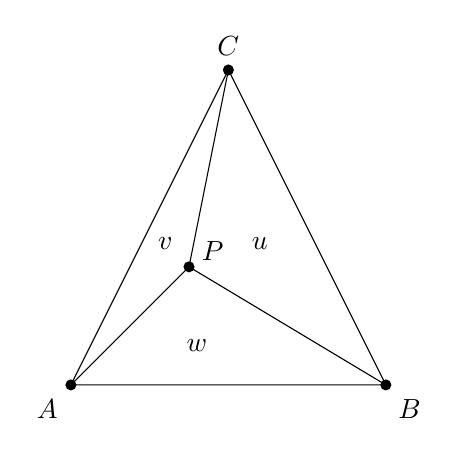
\begin{tikzpicture}
	
	\draw (0,0) -- (2,4) -- (4,0) -- (0,0);
	\fill (1.5,1.5) circle[radius=2pt];
	\fill (0,0) circle[radius=2pt];
	\fill (2,4) circle[radius=2pt];	
	\fill (4,0) circle[radius=2pt];	
	\draw (0,0) -- (1.5,1.5);
	\draw (2,4) -- (1.5,1.5);
	\draw (4,0) -- (1.5,1.5);
	
%	\draw (-0.3,-0.3) node {$(x_1,y_1)$};
%	\draw (4.3,-0.3) node {$(x_2,y_2)$};
%	\draw (2,4.3) node {$(x_3,y_3)$};
%	\draw (1.6,1) node {$(x,y)$};
	\draw (-0.3,-0.3) node {$A$};
	\draw (4.3,-0.3) node {$B$};
	\draw (2,4.3) node {$C$};
	\draw (1.8,1.7) node {$P$};
	
	\draw (1.6,0.5) node {$w$};
	\draw (2.4,1.8) node {$u$};
	\draw (1.2,1.8) node {$v$};
				
	\end{tikzpicture}
\end{center}

\begin{equation}
	\begin{aligned}
		u = \dfrac{\Delta BCP}{\Delta ABC}\\
		v = \dfrac{\Delta CAP}{\Delta ABC}\\
		w = \dfrac{\Delta ABP}{\Delta ABC}
	\end{aligned}
\end{equation}

\begin{equation}
f(x,y) = Uf(x_1,y_1)+Vf(x_2,y_2)+Wf(x_3,y_3)
\end{equation}

\subsubsection{Bilinear Interpolation}
\begin{center}


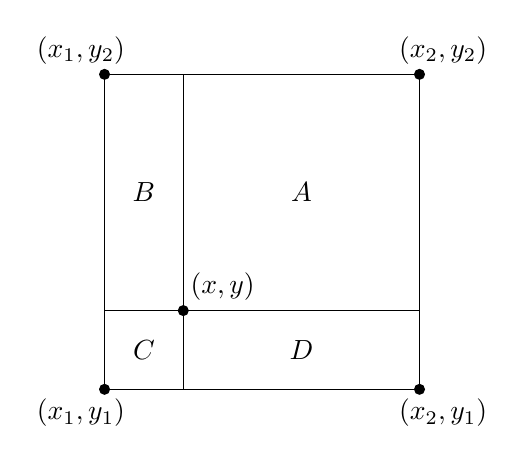
\begin{tikzpicture}

\draw (0,0) rectangle (4,4);
\draw (0,0) rectangle (1,1);
\draw (1,1) rectangle (4,4);
\fill (0,0) circle[radius=2pt];
\fill (0,4) circle[radius=2pt];
\fill (4,0) circle[radius=2pt];
\fill (4,4) circle[radius=2pt];
\fill (1,1) circle[radius=2pt];
\draw (-0.3,-0.3) node {$(x_1,y_1)$};
\draw (-0.3,4.3) node {$(x_1,y_2)$};
\draw (4.3,-0.3) node {$(x_2,y_1)$};
\draw (4.3,4.3) node {$(x_2,y_2)$};
\draw (1.5,1.3) node {$(x,y)$};
\draw (0.5,0.5) node {$C$};
\draw (0.5,2.5) node {$B$};
\draw (2.5,2.5) node {$A$};
\draw (2.5,0.5) node {$D$};

\end{tikzpicture}
\end{center}

\begin{equation}
	f(x,y) = Af(x_1,y_1)+Bf(x_2,y_1)+Cf(x_2,y_2)+Df(x_1,y_2)
\end{equation}
\subsection{Displacement Detection}
Least square correlation
%http://www.cs.umd.edu/~djacobs/CMSC426/Convolution.pdf
\begin{equation}
	\sum_{ij}^{} (c-d)^2
\end{equation}
\subsection{Importance Sampling}

\begin{center}
	
	
	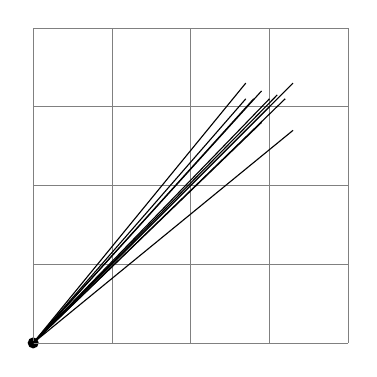
\begin{tikzpicture}
	\fill (0,0) circle[radius=2pt];
	\draw[step=1cm, gray, very thin] (0,0) grid (4,4); 
	\draw (0,0)	-- (3,3);
	\draw (0,0)	-- (2.7,3.3);	
	\draw (0,0)	-- (3.3,3.3);
	\draw (0,0)	-- (3.3,2.7);
	\draw (0,0)	-- (3.2,3.1);
	\draw (0,0)	-- (3.1,3.15);
	\draw (0,0)	-- (2.9,3.2);
	\draw (0,0)	-- (3,3.1);
	\draw (0,0)	-- (2.8,3.1);
	\draw (0,0)	-- (2.9,2.8);
	\draw (0,0)	-- (2.7,3.1);
	\end{tikzpicture}
\end{center}

\section{Evaluation Methods}
\chapter{Results and Discussion}
\chapter{Conclusion and Outlook}
\chapter{Acknowledgement}
\bibliography{References}
\chapter{Eidesstattliche Versicherung}
Ich versichere an Eides statt, dass ich diese Arbeit selbstständig verfasst und keine anderen als die angegebenen Hilfsmittel benutzt habe. Insbesondere habe ich keine im Literaturverzeichnis nicht genannten Internet-Quellen benutzt. Diese Arbeit habe ich vorher nicht in einem anderen Prüfungsverfahren eingereicht und die eingereichte schriftliche Fassung entspricht der Fassung auf dem elektronischen Speichermedium. Ich stimme einer Veröffentlichung dieser Arbeit zu.
\\
\\
\\
\\
\\
Simon Michel\\
Hamburg, \today
\end{document}

